%% Preâmbulo

\documentclass[12pt,tcc,abnt,latin,english,brazil]{df-ufpb}
\usepackage[lmargin=2.5cm,tmargin=2.5cm,rmargin=2.5cm,bmargin=2.5cm]{geometry} % margens da folha
\usepackage{tikz}
\usepackage{amssymb,amsthm,amsmath}
\newtheorem{theorem}{Teorema}[section]
\usepackage[style=abnt]{biblatex}
\addbibresource{amostra.bib}
\usepackage{lipsum}
%%% Metadados

\titulo{Investigações Sobre a Teoria das Superfícies Elásticas}
\subtitulo{Uma Crítica ao Métodos de Denis Poisson}
\autora{Sophie Germain}
\autorR{Germain, Sophie}
\orientador{Augustin-Louis Cauchy}
\chaves{análise real. equações diferenciais. mecânica do contínuo}
\keys{real analysis. differential equations. continuum mechanics}
\dia{13}
\mes{junho}
\ano{1821}
\linhadepesquisa{Matemática Aplicada}
\codigoBC{G15i}
\CDU{620.1}
\classi{Análise Real}
\classii{Equações Diferenciais}
\classiii{Mecânica dos Sólidos}

%% Corpo

\begin{document}

\capa
\publica
\rosto
\ficha
\begin{aprovacao}
  \membro{Prof. Dr. Jean-Baptiste Joseph Fourier}{Universidade de Paris}{Arguidor}
  \membro{Prof. Dr. Johann Carl Friedrich Gauss}{Universidade de Göttingen}{Arguidor}
\end{aprovacao}
\begin{dedicatoria}
à Isabel do Palatinado, com admiração  
\end{dedicatoria}

\begin{agradecimentos}
  Agradeço a meu pai, pelo apoio. Agradeço também a Lagrange e Gauss pelas cartas.
\end{agradecimentos}

\begin{resumo}
 Eu derivo uma equação diferencial adequada para a vibração de uma placa plana. Este resultado contribui para a mecânica newtoniana.
\end{resumo}

\begin{abstract}[Investigations on the Theory of Elastic Surfaces]{english}
  I derive a correct differential equation for the vibration of a plane lamina. This is a contribution to Newtonian mechanics.
\end{abstract}

\epigrafe[english]{Lock up your libraries if you like; but there is no gate, no lock, no bolt that you can set upon the freedom of my mind}{Virginia Woolf}{A Room of One’s Own}

\listadetabelas
\listadefiguras
\sumario


\chapter{Teoria dos Números}
Neste capítulo, apresento alguns resultados sobre números inteiros \autocite{gaussW8}.

\lipsum[1-3]


\begin{figure}
  \centering
  % A hexagon for memorizing trigonometric identities
  % Author: Josef Nilsen
  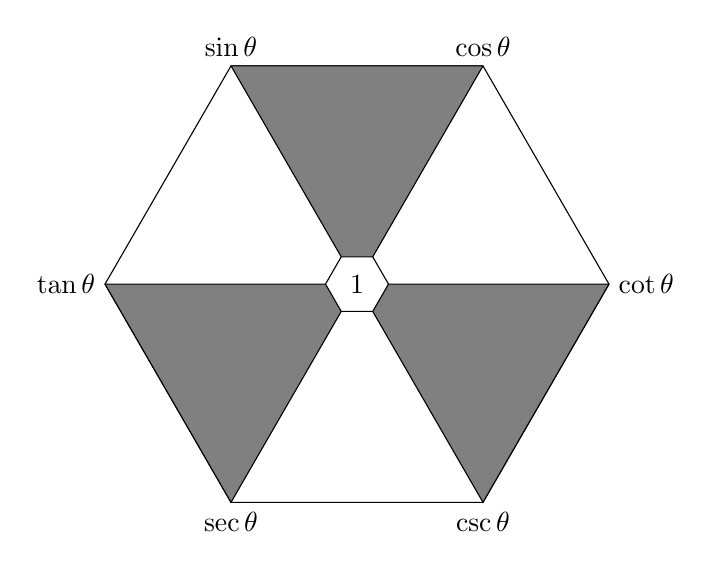
\begin{tikzpicture}[scale=4,cap=round,>=latex]
    % Radius of regular polygons
    \newdimen\R
    \R=0.8cm
    \coordinate (center) at (0,0);
    \draw (0:\R)
    \foreach \x in {60,120,...,360} {  -- (\x:\R) }
    -- cycle (300:\R) node[below] {$\csc \theta$}
    -- cycle (240:\R) node[below] {$\sec \theta$}
    -- cycle (180:\R) node[left] {$\tan \theta$}
    -- cycle (120:\R) node[above] {$\sin \theta$}
    -- cycle (60:\R) node[above] {$\cos \theta$}
    -- cycle (0:\R) node[right] {$\cot \theta$};
    \draw { (60:\R) -- (120:\R) -- (center) -- (60:\R) } [fill=gray];
    \draw { (180:\R) -- (240:\R) -- (center) -- (180:\R) } [fill=gray];
    \draw { (0:\R) -- (300:\R) -- (center) -- (0:\R) }  [fill=gray];
    \R=0.1cm
    \draw (0:\R) \foreach \x in {60,120,...,360} { -- (\x:\R) }
          [fill=white] -- cycle (center) node {1};
  \end{tikzpicture}

  \caption{Um hexágono}
\end{figure}

\lipsum[1-2]

\section{Sobre uma conjectura de Fermat}
Proponho o estudo de casos especiais da Conjectura de Fermat.

\begin{theorem}
  Seja $p$ um número primo ímpar. Caso exista um número primo auxiliar $q = 2np +1$, onde $n$ é um inteiro positivo que não é múltiplo de $3$, tal que:
  \begin{enumerate}
  \item se $x^{p} + y^{p} + z^{p} = 0 (\text{mod } q)$, então $q$ divide $zyz$
  \item $p$ não é o $p$-ésimo resíduo exponencial módulo $q$
  \end{enumerate}
  então a Conjectura de Fermat se aplica no caso $p$.
\end{theorem}

\lipsum[5-6]
\begin{quote}
  \lipsum[8-9]
  \autocite{ciceroFBM}
\end{quote}

\lipsum[1]

\section{Objeções}

\lipsum[7-9]

\chapter{Elasticidade}

Eu desenvolvo certas investigações iniciadas por \textcite{lagrangeO}.

\section{Observações finais}
\lipsum[1-7]

\begin{table}
  \centering
  \begin{tabular}{||c c c c||} 
    \hline
    Col1 & Col2 & Col2 & Col3 \\ [0.5ex] 
    \hline\hline
    1 & 6 & 87837 & 787 \\ 
    \hline
    2 & 7 & 78 & 5415 \\
    \hline
    3 & 545 & 778 & 7507 \\
    \hline
    4 & 545 & 18744 & 7560 \\
    \hline
    5 & 88 & 788 & 6344 \\ [1ex] 
    \hline
  \end{tabular}

  \caption{Tabela de valores}
\end{table}

\lipsum[1-3]

\printbibliography[heading=bibintoc,title=\bibname]{}

\end{document}
